\documentclass[11pt,a4paper]{article}
\usepackage[margin=22mm]{geometry}
\usepackage{fontspec,xeCJK,graphicx,booktabs,longtable,amsmath,placeins,hyperref,natbib}
\setmainfont{Times New Roman}
\setCJKmainfont{Noto Serif CJK SC}
\hypersetup{colorlinks=true,linkcolor=black,citecolor=black,urlcolor=blue}
\setlength{\emergencystretch}{4em}
\setlength{\parskip}{5pt}
\begin{document}
\title{Preserving nutrient objectives during uncertain fertilizer planning}
\date{}\maketitle
\begin{abstract}
Seasonal fertilizer decisions combine production, nitrogen-surplus and nutrient-use-efficiency objectives under uncertain weather. We examine how retaining these objectives during feasibility relaxation changes realized management, and whether a causal spatial prior improves transfer. Five typed numerical specialists couple a compact frozen response ensemble to nonanticipative weather-conditioned planning; an independent WOFOST81-SNOMIN referee supplies seasonal outcomes and daily mass-balance audits.

In the historical five-region benchmark of 52 former-held-out farm-years, equal-region joint compliance was 25.06\% for Sensorless Soft-Coupled, 21.58\% for Tier2-Composite, 4.00\% for archived bare relaxation and 27.00\% for masked Sensorless PPO. The paired Soft-Coupled-minus-PPO difference was -1.94 percentage points (marginal 95\% interval -8.55 to +4.09; full-family Holm-adjusted pooled farm-year sign-test p=1). The complete analysis covers 18,268 configurations, with seeds averaged within farm-year before inference and sources, cohorts and transfer schemes kept separate.

A first-pass decomposed spatial adapter slightly reduced row-pooled temporal-fold grain-N error, while world-equal and cross-region errors did not improve. Three-seed TRAIN-only physical readouts were positive in all 30 required region-target cells, with the weakest R² 0.0056. These are simulator-based, adaptively reused benchmark results, not prospective field assurance or proof of universal policy superiority.
\end{abstract}
\section{Introduction}
Nitrogen management is a sequential allocation problem embedded in crop growth, soil storage and weather variability. Production gains and fertilizer savings need to be interpreted alongside nutrient removal and nitrogen losses \cite{zhang2015}. A low seasonal surplus alone need not establish desirable management: crop removal can be sustained partly by depletion of soil nitrogen. We therefore retain a bilateral nutrient-use-efficiency corridor as well as a bounded surplus target \cite{eunep2015}.

Forecast feasibility and realized compliance are distinct. A controller can lack a candidate satisfying every conservative forecast constraint even though some actions remain agronomically reasonable. Once constraints are relaxed, the remaining ranking objective determines whether nutrient criteria continue influencing decisions. Comparing an objective-preserving controller with a profit-only fallback tests this decision mechanism under a common information and action interface.

A second challenge is spatial adaptation. High-dimensional environmental embeddings contain both persistent site differences and temporally varying information \cite{brown2025}. A low-rank projection of raw embeddings can largely reproduce site identity, while an out-of-distribution rejection can remove potentially useful seasonal information. Separating a physical soil baseline from a causal station-relative anomaly makes these roles explicit; successful admission of the anomaly does not by itself demonstrate predictive or management benefit.

Process-model evaluation provides controlled comparisons and exact bookkeeping, but cannot establish field validity by itself \cite{dewit2019} \cite{berghuijs2024}. We use it to ask three bounded questions: how objective retention affects management under matched information; where causal spatial adaptation helps or fails; and whether outputs and mechanistic readouts remain consistent with the frozen interfaces. We disclose the history of benchmark reuse and retain failed first-pass diagnostics rather than tuning their outcomes away.
\section{Methods}
The framework contains Spatial Twin, Climate, Eco Safety, Economics and Agronomic Control specialists. These are typed numerical modules, not conversational language-model agents. Specialists exchange public observations, candidate plans and numerical forecasts; the external physical referee is never exposed to a policy. Full-Telemetry includes contemporaneous leaf area, soil water and plant nitrogen. Sensorless masks these telemetry channels while retaining public crop stage, weather history, fertilizer history and static soil context. Agent decomposition is an implementation structure; modular-versus-monolithic equivalence does not identify an effect of agent count.

The response backbone maps 36 inputs through two 96-unit SiLU layers to yield, grain nitrogen and executed fertilizer nitrogen. Each 13,155-parameter network uses dropout 0.05; the deployed predictor averages three frozen seeds. Neural training and out-of-fold residual construction use TRAIN 1995–2009. No Phase8D neural retraining was performed. Five outer TRAIN year folds support physical readout diagnostics; all normalizers and stock-label regularization selection exclude their scored outer years.

Phase8D replaces an unbalanced random residual draw with deterministic region-by-stage quantile banks. Within each of 15 strata, joint three-output TRAIN residuals are sorted by signed surplus residual, partitioned into 32 bins and centered to zero mean. Candidate soil keys select the matching private bank; only unmatched synthetic soils use the region-equal global bank. For Phase8D planning metrics, every weather branch integrates all 32 residual members with product weights, retaining the joint residual vector. Quantile and upper-tail calculations in distribution\_metrics use this full weighted measure. The frozen Sensorless PPO comparator retains its registered 91-D observation construction and normalization, including 32 systematic weather-residual pair summaries. It receives the repaired causal forecasts and residual banks but is not retrained. Thus the comparison matches information access and action constraints, not every distributional preprocessing operation; differences cannot be attributed solely to optimization or agent organization.

Climate analog matching uses only observations available at the decision date and a TRAIN archive. Scenario warming is removed from the observed-history temperature before matching and before the baseline forecast, while future scenario descriptors retain the prescribed warming and carbon-dioxide regime. Source relative humidity is preserved consistently with the training feature contract. The idealized +1.8°C and +3.5°C settings are stress scenarios, not operational numerical weather forecasts. Information partitions reveal seven-day rain and then temperature; the current action is shared across all branches. Nodewise nonanticipativity does not establish global chance-constrained or CVaR optimality.

The operational action set is 0, 10, 20, 40, 60, 80 or 100 kg N/ha, subject to the common stage scheduler and cumulative fertilizer budget. Surplus is total seasonal nitrogen input minus grain nitrogen removal; total input contains fertilizer, seed and wet deposition, excluding initial soil stocks. NUE is grain nitrogen divided by that input. Realized joint compliance requires 0.50 ≤ NUE ≤ 0.90 and 0 ≤ surplus ≤ cap. Native nitrogen loss is bottom leaching plus denitrification, evaluated separately from surplus. Partial profit equals grain revenue minus fertilizer cost plus experimental compliance subsidy minus any specified surplus tax; it excludes other production costs.

The coupled ranking score is partial profit plus 250 times active joint probability minus 300 times normalized corridor distance. Upper NUE violation receives weight 1.5, and surplus distance includes a 2 kg N/ha interior margin. Tier2-Composite first applies strict active forecast masks; if empty, it prefers candidates preserving both the mean-surplus corridor and bilateral NUE safety, then falls back to the archived upper-surplus condition. Soft-Coupled ranks the same legal candidates continuously without hard-tail masks. Archived bare relaxation preserves its profit-only fallback for comparator faithfulness. Operational zero after OOD rejection or an empty set is not labelled compliance.

G1 calibrates signed two-sided conformal corrections on Dev 2010–2014 and evaluates cross-year macro coverage, Brier skill and ranking regret. An approved, explicitly versioned amendment compares actual calibrated interval width, rather than signed correction alone, because different base quantile widths make the signed correction unsuitable as a sharpness measure. The original failed signed-offset verdict remains archived. This amendment uses frozen predictions, with zero additional Dev access or model changes. Pooled calibration and macro coverage are different summaries; marginal empirical coverage is not a conditional regional guarantee.

For spatial transfer, Stage A always supplies a standardized Static3 physical-soil Ridge correction. Stage B uses a 64-D satellite anomaly relative to that station's unlabelled historical mean through the available t−1 embedding year. It uses neither future satellite years nor held-out outcome labels. Weighted PCA has rank at most four; accepted anomalies contribute an additional residual Ridge correction, while anomaly rejection falls back to Static3. LOYO removes the entire scored calendar year across sites; LORO removes the scored region. The first-pass inner-year grid and fits remain frozen after outer results were observed. A later proposed grid expansion and Dev threshold change were withdrawn; neither was executed.

The evaluation retains 18,268 configurations, the complete 180-cell climate-cap-price-subsidy stress surface, and the 90-cell continuity subset. Every policy recomputes its actions. Verified historical physical terminals can be reused only along exact dated requested-action paths after native recovery of the public observation prefixes; old policy traces are not substituted. Unknown paths run the unchanged native WOFOST81-SNOMIN referee. An infrastructure-only P2 path-name failure stopped the first attempt after 1,915 completed configurations; an explicit hash-verified recovery preserved those records and corrected only the loader mapping. Daily absolute N and C residual tolerances are 1e−10 and 1e−9 kg/ha.

PPO seeds are averaged within farm-year before paired inference. Primary campaign and predictive cohort summaries keep NASA/WUR sources, Former-Held-Out/Public-Reused cohorts and LOYO/LORO schemes separate. The original mixed 44-site-year predictive aggregate is explicitly labelled archival. Effects and descriptive intervals use equal-region weighting with paired years resampled within region. Exact sign-test probabilities use pooled paired farm-year signs, not a region-weighted test of the equal-region mean. Every reported exact two-sided sign test belongs to one Holm family \cite{holm1979}. Marginal confidence intervals are not simultaneous confidence bands. Reused evaluation data constrain interpretation \cite{cawley2010} \cite{roberts2017}: the campaign is an adaptive benchmark evaluation and P2 is retrospective causal transfer, not a new prospective blind test.
\begin{figure}[p]\centering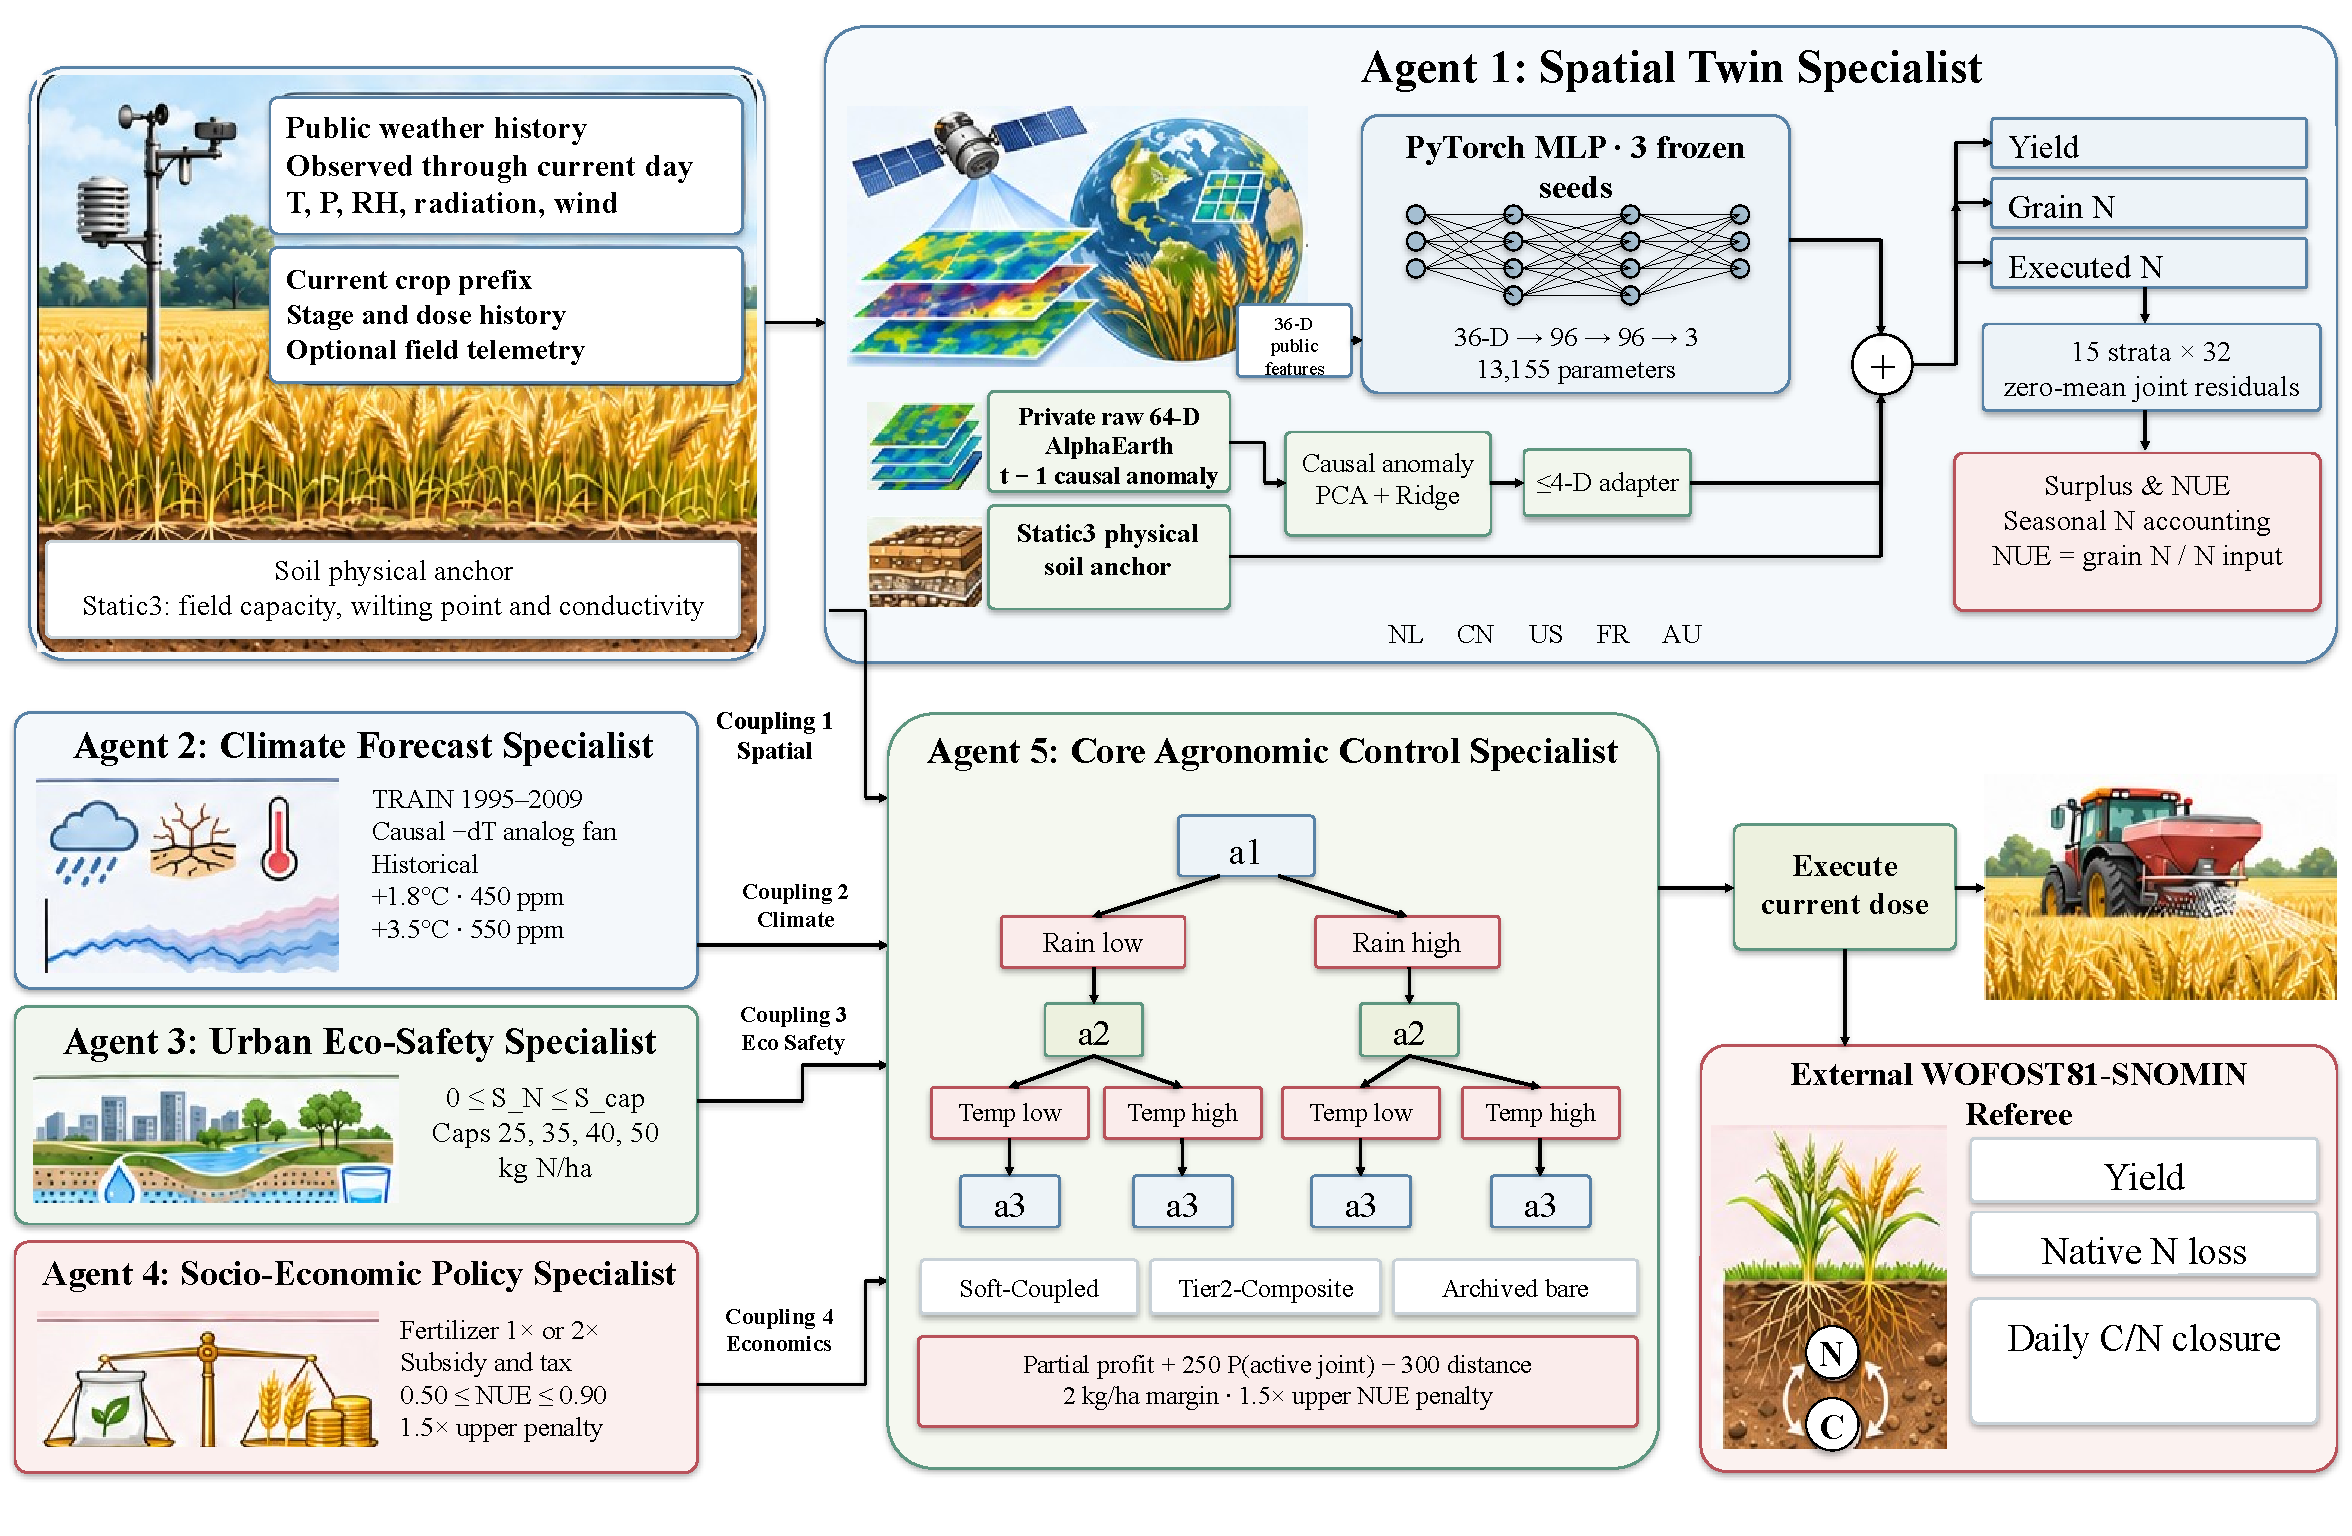
\includegraphics[width=\textwidth]{../../reports/phase8/figures/fig1-architecture.pdf}\caption{Five numerical specialists, a frozen three-seed response ensemble, causal Static3-plus-anomaly adaptation, full weather × 32 residual integration and an external physical referee. No hidden referee state enters policy decisions.}\label{fig:1}\end{figure}\FloatBarrier
\section{Results}
At the historical reference cap of 40 kg N/ha, Sensorless Soft-Coupled reached 25.06\% joint compliance, compared with 21.58\% for Tier2-Composite and 4.00\% for archived bare relaxation. Their equal-region partial profits were 887.77, 883.85 and 976.24 EUR/ha, respectively. Full-Telemetry Soft-Coupled reached 17.94\%. These averages describe the registered five-region mixture; regional results are reported separately in Figure 2 and the complete summary tables.

Masked Sensorless PPO reached 27.00\% joint compliance. The paired difference relative to Soft-Coupled was -1.94 percentage points (marginal 95\% interval -8.55 to +4.09; full-family Holm-adjusted pooled farm-year sign-test p=1). All 13,512 exact sign-test contrasts share the same Holm family. Neither a favorable mean nor an unadjusted comparison establishes general superiority. The five former-held-out Netherlands years also limit the resolution of an exact two-sided paired sign test to a minimum attainable p of 0.0625.

G1 cross-year macro 90\% coverage was 90.78\% for Full-Telemetry and 90.37\% for Sensorless. Both tracks had positive surplus-event Brier skill against ExtraTrees and climatology at caps 25, 35, 40 and 50, with ranking regret below ExtraTrees. Full and Sensorless regrets were 3.666 and 4.757 EUR/ha. Calibrated mean interval widths were 62.504 and 69.533 kg N/ha, although signed corrections were −5.740 and −6.781 kg N/ha. Regional coverage was heterogeneous: Full-Telemetry AU coverage was 75.19\%, so the macro result cannot be treated as a regional assurance.

The first-pass Dev closed-loop diagnostic contained 300 configurations and 84 native trajectories. At AU cap 25, Soft-Coupled realized compliance in 40\% of Full-Telemetry and 20\% of Sensorless years, while Tier2-Composite Sensorless remained at zero. Full-Telemetry Netherlands mean doses were 214, 218 and 218 kg N/ha at caps 25, 35, 40. These fixed observations motivate no further threshold tuning and do not establish a monotonic dose response between every pair of caps.

Equal-region spatial closed-loop comparisons remained stratified: Former-Held-Out LOYO (n=40): Full64 29.83\%, Static3 27.61\%; Former-Held-Out LORO (n=40): Full64 20.39\%, Static3 17.89\%; Public-Reused LOYO (n=4): Full64 25.00\%, Static3 25.00\%; Public-Reused LORO (n=4): Full64 25.00\%, Static3 25.00\%. Cohort-separated predictive results were: Former-Held-Out LOYO (n=40): Full64/Static3 row-pooled MSE 452.02/454.04, world-equal MSE 445.83/442.19; Full64 predictive acceptance 88.36\% of rows and 77.50\% world-equal; Former-Held-Out LORO (n=40): Full64/Static3 row-pooled MSE 494.84/481.10, world-equal MSE 517.65/505.15; Full64 predictive acceptance 72.02\% of rows and 60.00\% world-equal; Public-Reused LOYO (n=4): Full64/Static3 row-pooled MSE 549.91/556.60, world-equal MSE 549.91/556.60; Full64 predictive acceptance 100.00\% of rows and 100.00\% world-equal; Public-Reused LORO (n=4): Full64/Static3 row-pooled MSE 586.98/583.26, world-equal MSE 586.98/583.26; Full64 predictive acceptance 100.00\% of rows and 100.00\% world-equal. These are prediction-row diagnostics, distinct from acceptance across realized policy decisions. The original all 44 mixed-cohort predictive diagnostic, retained as an archival aggregate rather than an unpooled result, gave LOYO Full64 grain-N MSE 462.87 versus Static3 465.41, with 89.65\% row-level prior acceptance. World-equal LOYO MSE was 455.29 versus 452.59, so the small row-pooled gain was not invariant to weighting. In LORO, Full64 acceptance rose to 75.12\% of rows, or 63.64\% under world-equal weighting, but predictive MSE was 505.05 versus Static3 492.41 (RMSE 22.47 versus 22.19 kg N/ha). Admission therefore improved without proving cross-region predictive benefit. No grid expansion or outer-result-dependent refit was used.

The world-weighted, nested TRAIN physical probe achieved positive within-region out-of-fold R² in all 30 required cells across organic nitrogen, soil carbon and net mineralization. The minimum was 0.0056 for Sensorless US soil carbon. Organic nitrogen and net mineralization are algebraically linked under the simulated stock balance, so those two readouts are not independent mechanistic validations. Other diagnostics, including nitrogen-loss decoding, may remain negative; complete target-level results are retained. Backbone weights were unchanged and the proposed neural auxiliary-head experiment was explicitly skipped.

All 18,268 scored configurations passed the daily mass audit. Maximum absolute N and C residuals were 1.904e-11 and 2.115e-10 kg/ha. The campaign performed 1,886 actual native simulations and 16,382 verified trajectory replays. Every replay retained fresh policy decisions and a case-specific trace. Figure 4 displays all 180 registered stress cells, including unfavorable cells; idealized climate responses are descriptive simulator sensitivities.
\begin{longtable}{llrrr}
\caption{Equal-region results at the historical reference setting.}\\
\toprule Configuration & Track & n & Joint (\%) & Profit (EUR/ha)\\\midrule\endfirsthead
\toprule Configuration & Track & n & Joint (\%) & Profit (EUR/ha)\\\midrule\endhead
DVS-N2 tree & Full & 52 & 26.73 & 885.74\\
LegacyV6Full tree & Full & 52 & 20.21 & 890.84\\
LegacyV6PPO tree & Full & 52 & 20.54 & 902.35\\
SensorlessPPO tree & Sensorless & 52 & 27.00 & 890.32\\
TreeExtraTrees soft & Full & 52 & 21.58 & 879.77\\
TreeExtraTrees tree & Full & 52 & 21.58 & 881.87\\
TreeExtraTrees soft & Sensorless & 52 & 18.09 & 879.73\\
TreeExtraTrees tree & Sensorless & 52 & 16.42 & 878.33\\
TreeLinear soft & Full & 52 & 20.06 & 890.15\\
TreeLinear tree & Full & 52 & 20.06 & 889.17\\
TreeLinear soft & Sensorless & 52 & 14.45 & 890.45\\
TreeLinear tree & Sensorless & 52 & 14.45 & 890.45\\
TreeMLP greedy-frozen & Full & 52 & 25.06 & 886.70\\
TreeMLP hard-bare-tier2 & Full & 52 & 9.67 & 970.59\\
TreeMLP open-loop & Full & 52 & 21.58 & 884.53\\
TreeMLP soft & Full & 52 & 17.94 & 885.40\\
TreeMLP tree & Full & 52 & 23.39 & 884.17\\
TreeMLP greedy-frozen & Sensorless & 52 & 16.42 & 887.73\\
TreeMLP hard-bare-tier2 & Sensorless & 52 & 4.00 & 976.24\\
TreeMLP open-loop & Sensorless & 52 & 19.91 & 882.43\\
TreeMLP soft & Sensorless & 52 & 25.06 & 887.77\\
TreeMLP tree & Sensorless & 52 & 21.58 & 883.85\\
TreeWeather soft & Full & 52 & 17.94 & 886.00\\
TreeWeather tree & Full & 52 & 16.12 & 883.86\\
TreeWeather soft & Sensorless & 52 & 17.94 & 886.00\\
TreeWeather tree & Sensorless & 52 & 16.12 & 883.86\\
remove-climate soft & Full & 31 & 20.91 & 875.90\\
remove-climate tree & Full & 31 & 24.24 & 875.70\\
remove-climate soft & Sensorless & 31 & 17.58 & 872.98\\
remove-climate tree & Sensorless & 31 & 22.42 & 872.21\\
remove-eco soft & Full & 52 & 12.48 & 884.57\\
remove-eco tree & Full & 52 & 12.48 & 884.57\\
remove-eco soft & Sensorless & 52 & 14.30 & 886.63\\
remove-eco tree & Sensorless & 52 & 14.30 & 884.42\\
\bottomrule\end{longtable}
\begin{figure}[p]\centering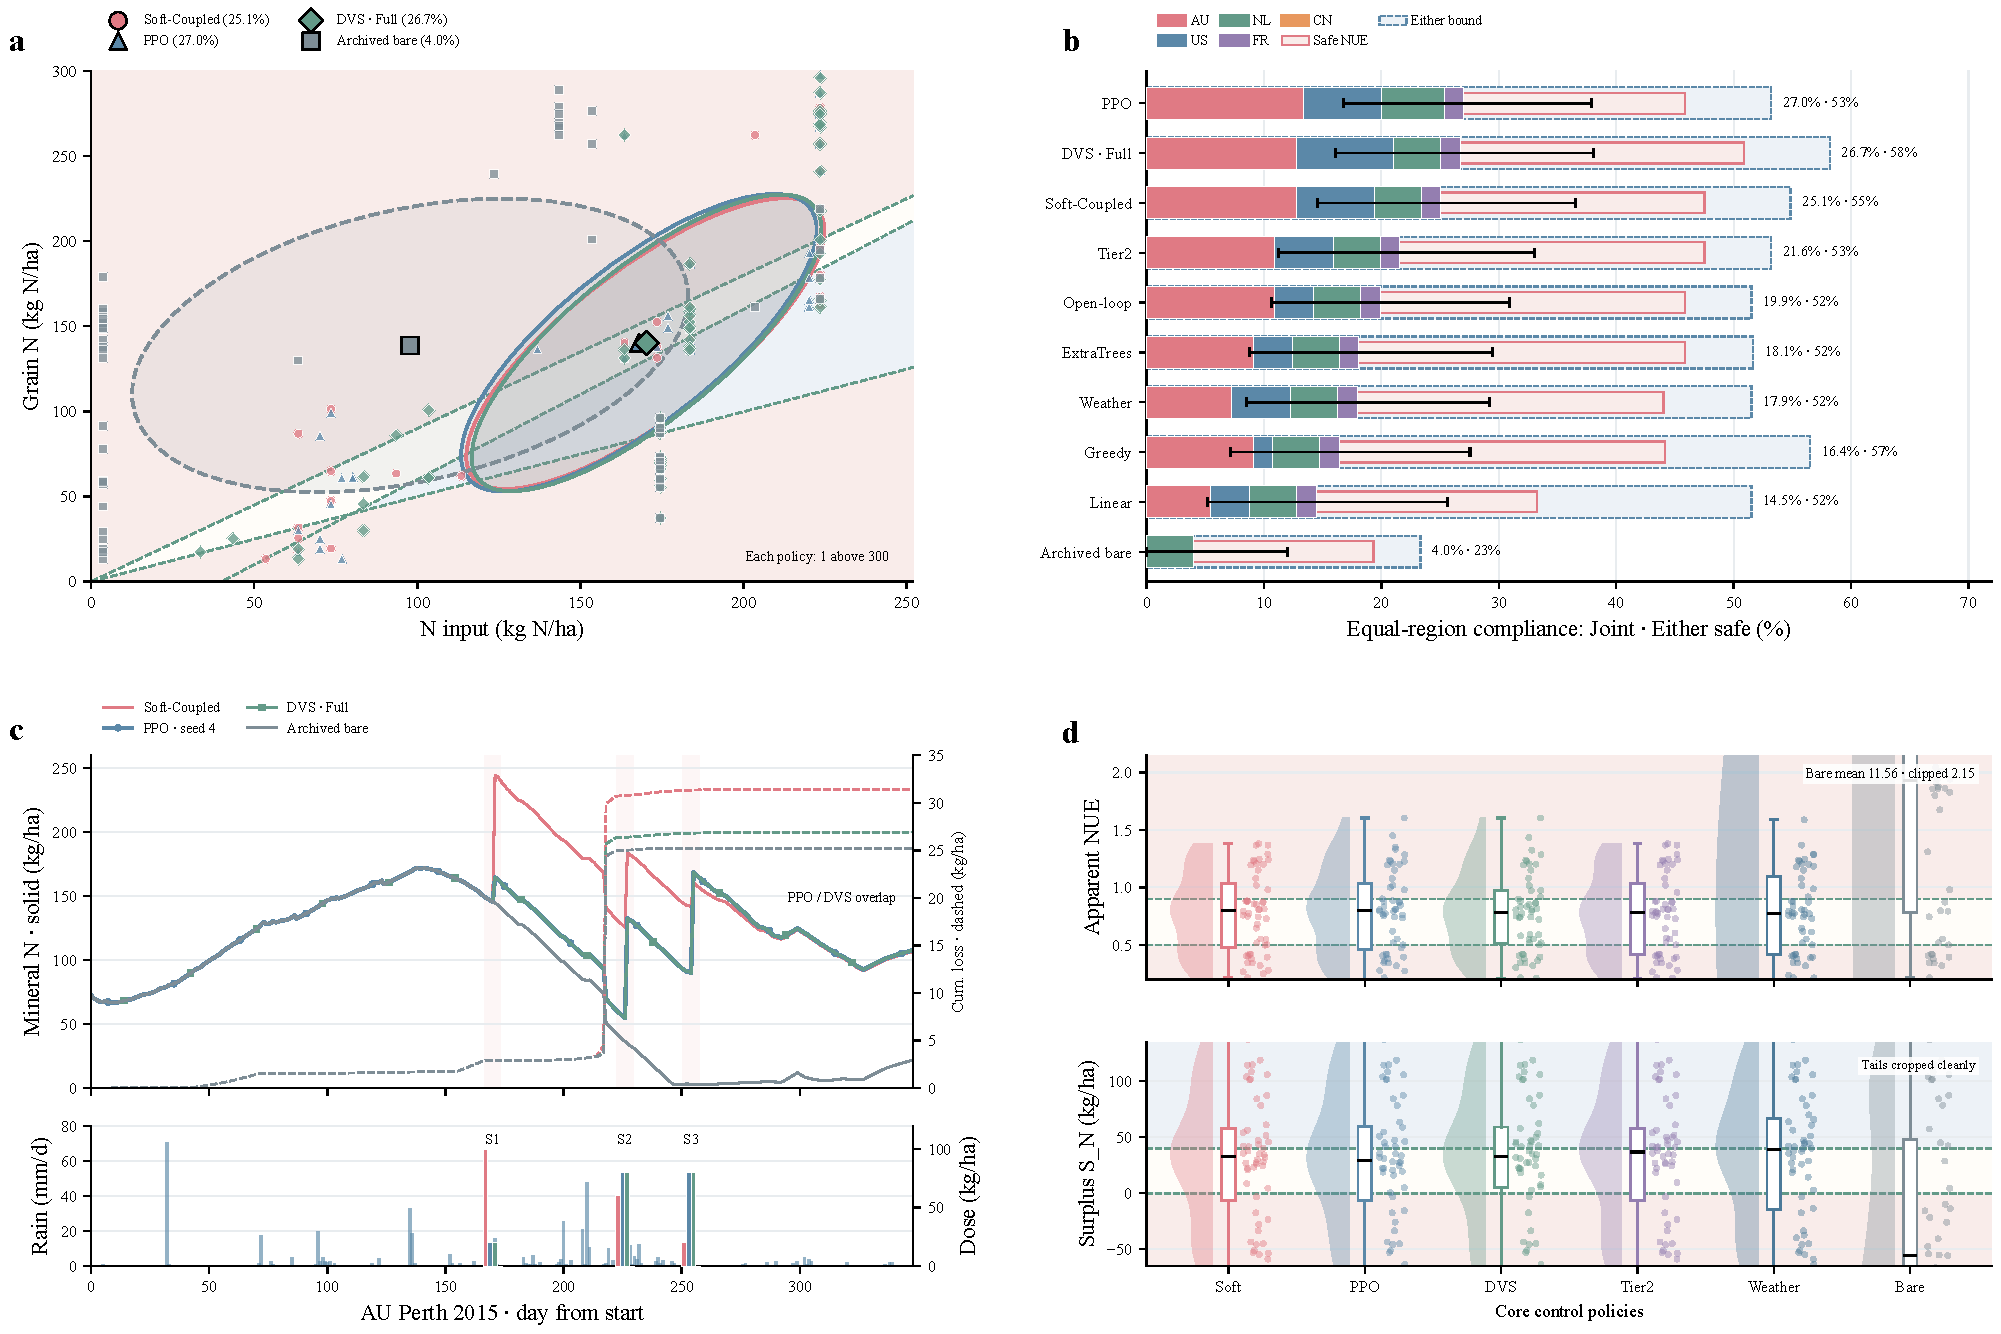
\includegraphics[width=\textwidth,height=.78\textheight,keepaspectratio]{../../reports/phase8/figures/fig2-p1-regimes.pdf}\caption{P1 historical reference comparisons under matched information. Soft-Coupled, strict Tier2-Composite and archived bare relaxation are kept distinct; regional heterogeneity and nitrogen-mining indicators accompany compliance.}\label{fig:2}\end{figure}\FloatBarrier
\begin{figure}[p]\centering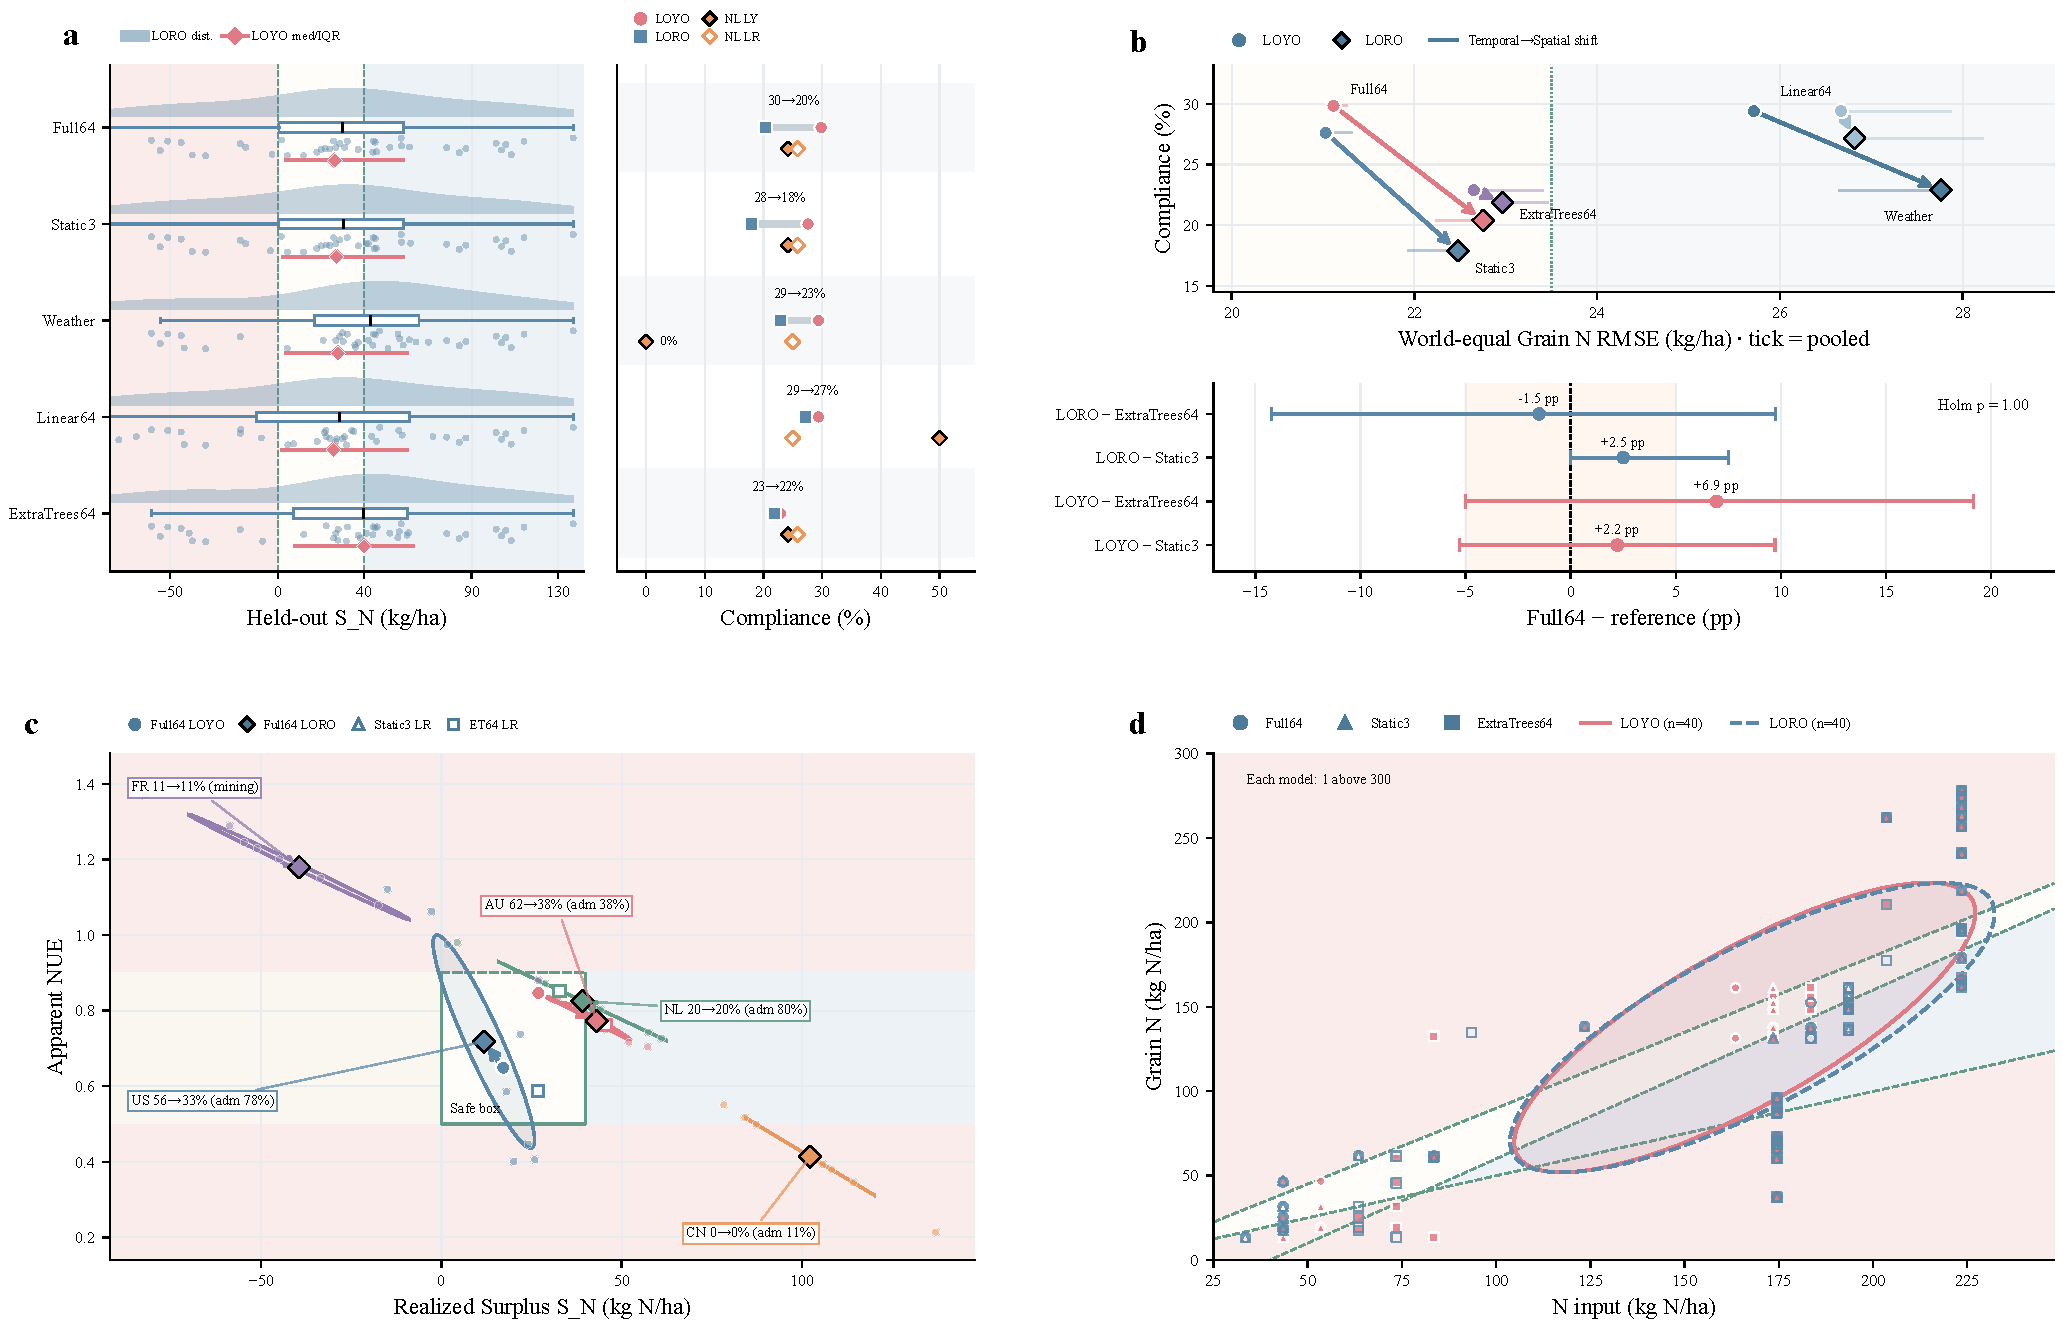
\includegraphics[width=\textwidth,height=.78\textheight,keepaspectratio]{../../reports/phase8/figures/fig3-p2-transfer.pdf}\caption{P2 closed-loop transfer: panel a shows all four Former/Public-by-LOYO/LORO strata; regional panels use Former only. Panel c pools closed-loop decision counts within the Former cohort, distinct from predictive-row acceptance. Anomaly OOD falls back to Static3. Acceptance does not guarantee predictive improvement.}\label{fig:3}\end{figure}\FloatBarrier
\begin{figure}[p]\centering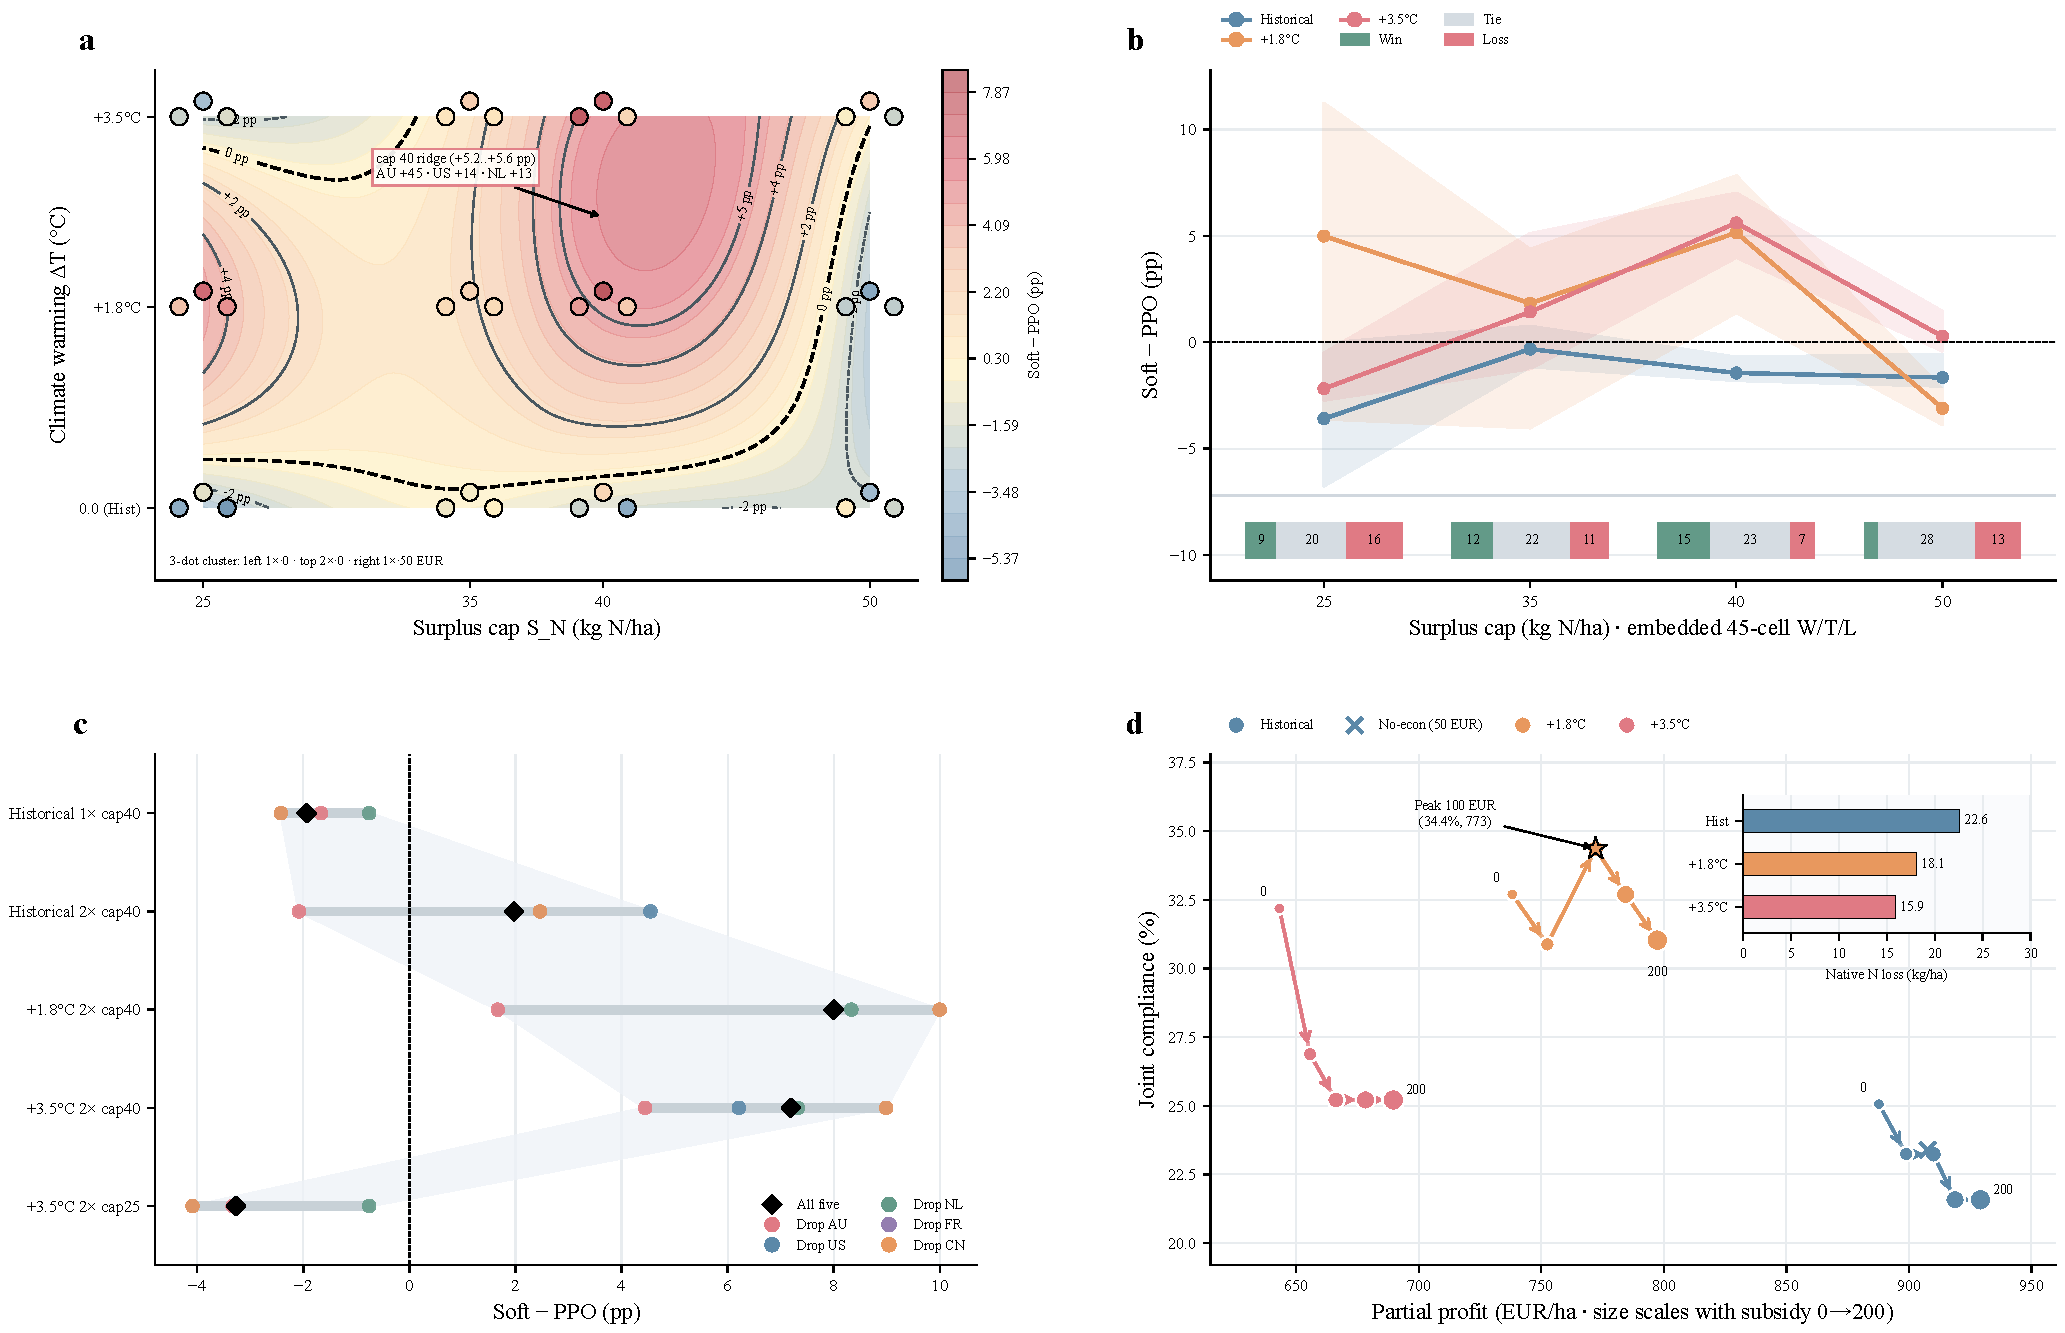
\includegraphics[width=\textwidth,height=.78\textheight,keepaspectratio]{../../reports/phase8/figures/fig4-factorial-stress.pdf}\caption{Complete 180-cell climate-cap-price-subsidy stress surface. Black outlines mark 90 continuity cells. Heatmaps retain unfavorable cells and idealized climates are not operational forecasts.}\label{fig:4}\end{figure}\FloatBarrier
\begin{figure}[p]\centering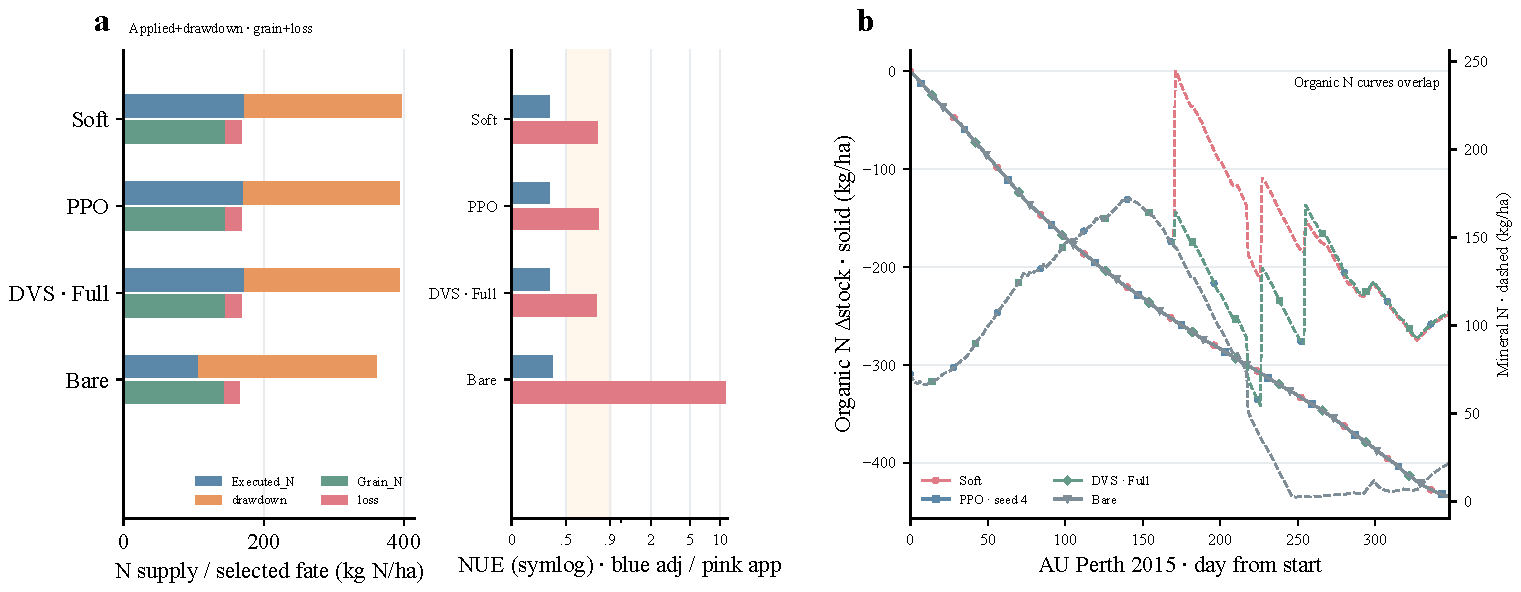
\includegraphics[width=\textwidth,height=.78\textheight,keepaspectratio]{../../reports/phase8/figures/fig5-deployment-closure.pdf}\caption{Frozen compact model and interface, case-configuration daily mass closure, actual native simulation count and verified trajectory replay count. Repeated configuration-day records are not independent seasons.}\label{fig:5}\end{figure}\FloatBarrier
\section{Discussion}
Objective retention, forecast conservatism and spatial prior admission address different failure modes. The soft and hard-composite designs share a score but apply different feasibility mechanisms. A narrow bilateral corridor can exclude an action near a forecast threshold, whereas continuous penalties preserve a graded preference. The untuned AU contrast illustrates this distinction; it does not identify a universal advantage of continuous relaxation across climates, crops or threshold choices.

Zero-centering residual banks removes an accidental mean shift, while retaining all weather-residual combinations avoids losing rare branch mass through index pairing. These are distributional consistency repairs. Centering does not prove the residual law is conditionally correct, and finite region-stage quantiles are not a complete account of uncertainty. Likewise, correcting the CQR sharpness comparison does not repair regional undercoverage or establish field safety. Those boundaries remain visible rather than being hidden behind a passing macro gate.

Decomposing the spatial prior separates physical-soil adaptation from temporal satellite novelty. The first-pass LORO results show that positive anomaly acceptance and improved prediction need not coincide. A satellite embedding is a compressed environmental descriptor, not a direct soil-stock or management observation. The retained cross-region error increase is therefore a meaningful boundary of this particular frozen anomaly-transfer design. Further regularization studies would be exploratory development and require new confirmatory evidence.

The physical readouts test whether seasonal stock variation is linearly accessible from frozen response features. Region-specific intercepts and world-scaled penalties avoid mistaking between-region stock baselines or repeated plan rows for independent seasonal information. Nested year selection and seed-specific prediction averaging improve the diagnostic without changing the online controller. The near-zero Sensorless US carbon result remains weak evidence, and linked organic-N/mineralization targets must not be counted as independent confirmation. No latent readout demonstrates causal identification of hidden soil state.

The benchmark contains multiple information tracks, policies and weather regimes but remains simulator-based and adaptively reused. Source-specific weather, crop parameterization, soil inputs and fixed prices constrain extrapolation. Partial profit is not whole-farm welfare; prescribed warming is not a downscaled climate projection; macro coverage is not conditional regional coverage. Future field validation should prospectively freeze decisions and analysis before new observations, include operational forecast error and measurement costs, and retain both favorable and unfavorable regional outcomes.
\section{Conclusion}
Phase8D repaired residual integration, warming alignment, relaxation scoring, spatial-prior decomposition and physical-readout regularization while keeping neural weights and first-pass Dev/P2 decisions frozen. The resulting Sensorless Soft-Coupled historical joint compliance was 25.06\%, with the complete paired and multiplicity-adjusted comparisons reported alongside regional heterogeneity. Causal prior admission improved but did not eliminate cross-region prediction error. The evidence supports a reproducible comparison of objective-preserving decision designs within this simulator benchmark; prospective agronomic effectiveness remains to be established.
\clearpage\appendix
\section{Evidence and reproducibility}
All Phase8B/C reports, figures and manuscript history remain archived. Phase8D uses first-pass frozen controllers and adapters with explicit CQR width amendment and adaptive benchmark reuse disclosure. Original PPO ZIP containers were unavailable; separately versioned TRAIN-only reconstructions remain unchanged. All new policy decisions are recomputed. Complete summaries, all contrasts and daily mass audits accompany the draft. No submission is authorized.
\clearpage\bibliographystyle{plainnat}\bibliography{references}\end{document}